\chapter{Úvod}

Stavebnice \lego{ }je jedna z nejznámějších a nejprodávanějších stavebnicí na světě. 

% * <paral.jarek@gmail.com> 2017-04-27T12:46:22.004Z:
% 
% > Stavebnice
% Testovací komentář.
% Komentáře lze přidávat pomocí "+" v horní nabídce.
% 
% ^ <paral.jarek@gmail.com> 2017-04-27T12:46:45.502Z:
% 
% A testovací odpověď.
% 
% ^ <lucie.karmova@jcmm.cz> 2017-04-27T13:01:57.651Z:
%
% Brekeke.
%
% ^ <paral.jarek@gmail.com> 2017-04-27T14:00:55.322Z.

V nabídce firmy \lego{ }je i robotický set s názvem \legoM. 
% * <lucie.karmova@jcmm.cz> 2017-04-27T13:01:31.014Z:
% 
% > mají
% Kdo mají? Firma LEGO?
% Navrhuju: V nabídce firmy LEGO je i robotický set s názvem
% 
% 
% ^ <paral.jarek@gmail.com> 2017-04-27T13:14:27.014Z:
%
% Chtěl jsem se vyhnout použití slova LEGO, ale asi to tady bez něj nepůjde.
%
% ^.
Dle oficiálních údajů se jedná historicky nejprodávanější set z celé nabídky firmy~\cite{legoGizmodo_SalesStatistic}. 
To je také jeden z hlavních důvodů, proč se tato práce věnuje této stavebnici. 
%To je také jeden z hlavních důvodů, proč je tato práce zaměřena na tuto stavebnici. 

Z výše uvedených informací vyplývá, že jde pravděpodobně o nejdostupnější robotickou stavebnici na světě (pokud pomineme platformu \arduino, která je ovšem zaměřena na jinou skupinu lidí -- lidí, kteří se nebojí elektroniky, elektronických obvodů, složitějších návrhů konstrukce, atd.).
% * <lucie.karmova@jcmm.cz> 2017-04-27T13:04:12.937Z:
% 
% > jedná
% Přeformuluj, ve 3 řádcích máš 3 x slovo "jedná".
% 
% ^ <paral.jarek@gmail.com> 2017-04-27T13:12:29.824Z:
%
% Hotovo.
%
% ^ <paral.jarek@gmail.com> 2017-04-27T14:01:00.658Z.

\begin{figure}[h]
	\centering
	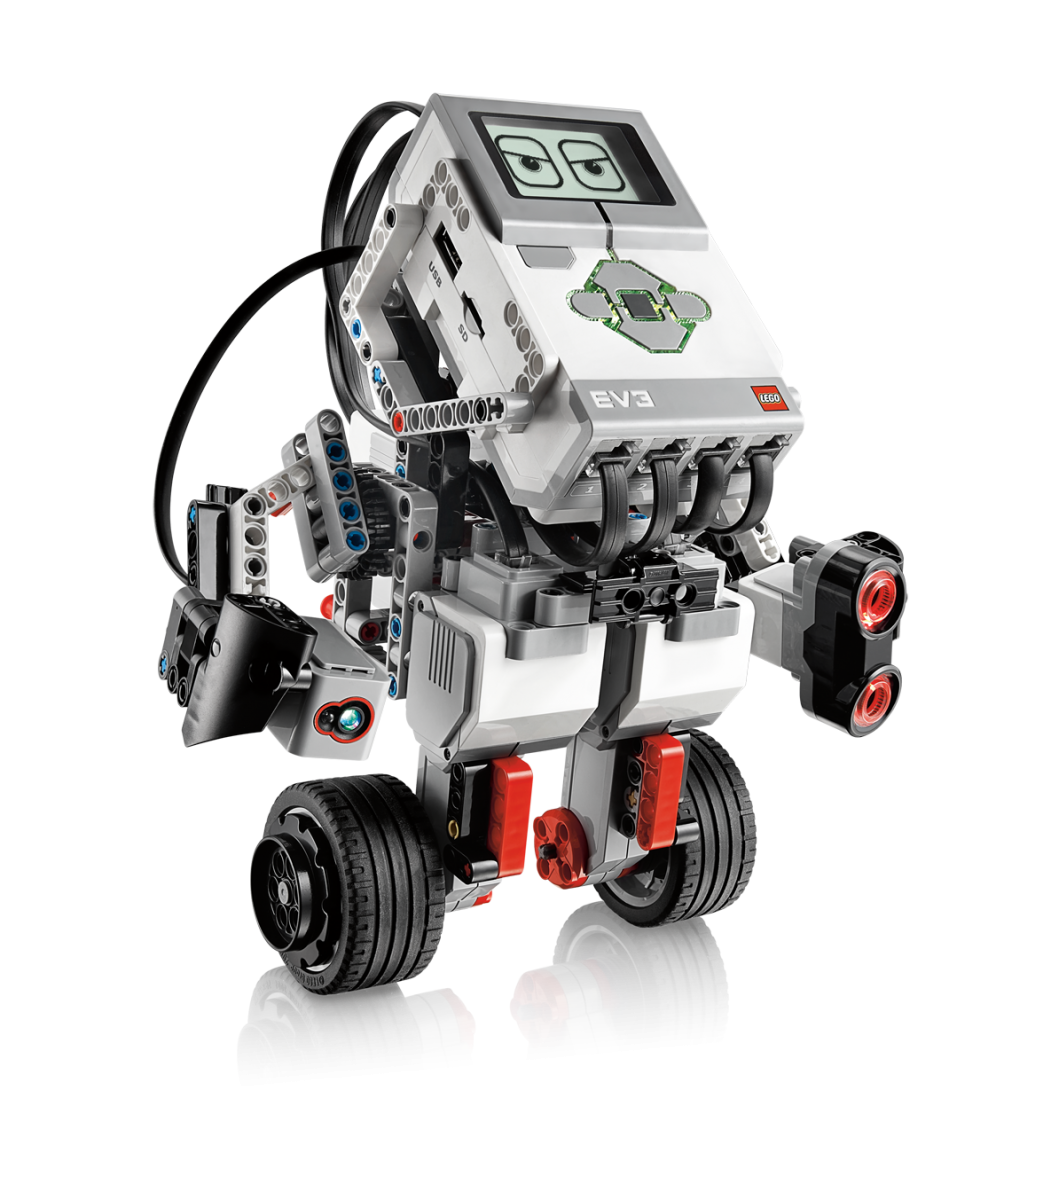
\includegraphics[width=250px]{images/lego-mindstorms-ev3_Robotics-for-Kids.png}
	\caption[\legoEV{ }-- samobalancující robot]{\legoEV{ }-- samobalancující robot\protect\footnotemark}
	\label{fig:lego-mindstorms-ev3_Robotics-for-Kids}
\end{figure}


\footnotetext{Zdroj: \url{https://www.bermotech.com/training/coding-for-teenagers-and-children/y-robotics-with-lego-mindstorm-ev3/}}

\begin{figure}[h]
	\centering
	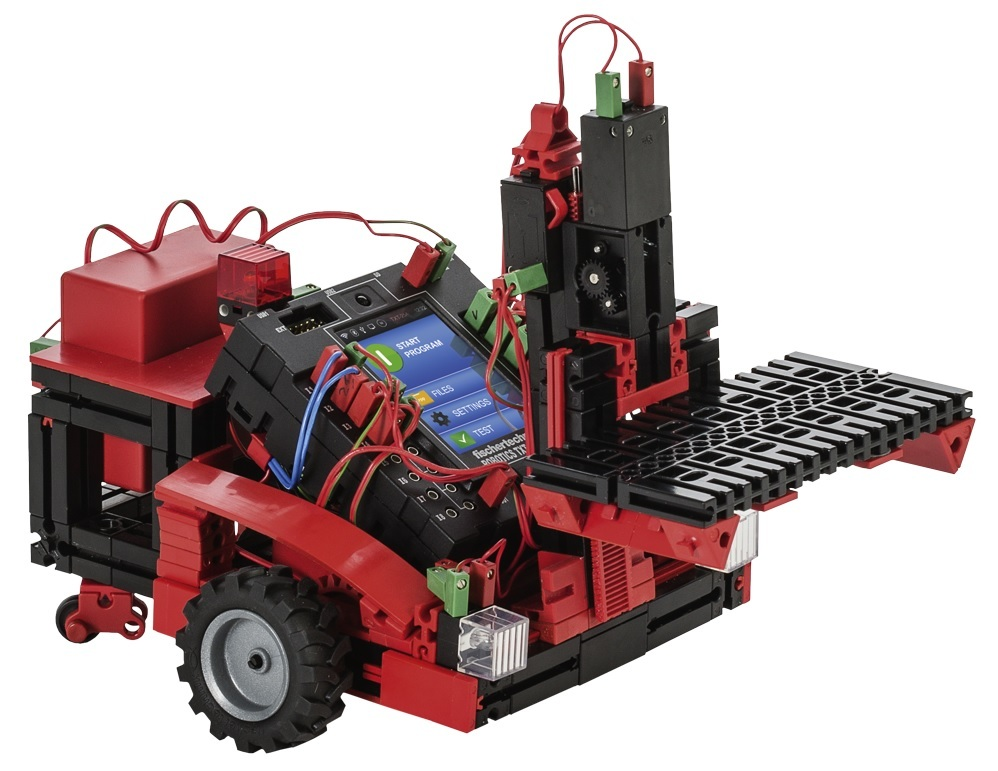
\includegraphics[width=250px]{images/fischertechnik_ROBO-TX-Explorer_02.jpg}
	\caption[Fischertechnik -- ROBO TX Explorer]{Fischertechnik -- ROBO TX Explorer\protect\footnotemark}
	\label{fig:fischertechnik_ROBO-TX-Explorer}
\end{figure}

\footnotetext{Zdroj: \url{http://www.helago-cz.cz/eshop-519143-workstation-robo-tx-training-lab-tx-explorer-146560.html}}

Existuje i mnoho podobných stavebnic~\cite{intorobotics_BestAlternativesToLegoMindstormsKits}. 
Například \fischerT prodává podobné robotické sety jako \lego{~}\cite{fischertechnik_ROBOTICS}. 
% * <lucie.karmova@jcmm.cz> 2017-04-27T13:06:18.621Z:
% 
% > prodává
% Slepená slova.
% 
% ^ <paral.jarek@gmail.com> 2017-04-27T13:17:53.886Z:
%
% A to je špatně nebo ok? :-)
%
% ^.
Uživateli nabízí rozsáhlejší pohled do elektroniky a fungování jednotlivých modulů. 
Umožňuje také relativně snadno přidat vlastní moduly.
Zároveň má jednoduché grafické programovací prostředí podobně jako \lego. 
\FischerT{ }ovšem není tak rozšířen jako \legoM, protože ačkoliv nabízí v některých ohledech více funkcí, zároveň klade větší nároky na uživatele, je podstatně dražší (základní set~\cite{fischertechnik_HelagoEshop_ROBOTICS-TXT-COMPETITION-SET} stojí cca dvakrát tolik co \legoEV{ Základní souprava}~\cite{lego_eduxeEshop_CoreSet}) a nemá takový věhlas a značku.
% * <lucie.karmova@jcmm.cz> 2017-04-27T13:09:08.477Z:
% 
% > cca.
% Za cca nepatří tečka, viz http://prirucka.ujc.cas.cz/?id=780
% 
% ^ <paral.jarek@gmail.com> 2017-04-27T13:17:22.584Z:
%
% Tak to jsem to doteď psal všude špatně :-(. Pamatoval jsem si jen "viz".
%
% ^ <paral.jarek@gmail.com> 2017-04-27T13:18:26.453Z:
%
% Opraveno.
%
% ^ <paral.jarek@gmail.com> 2017-04-27T14:00:46.559Z.
% * <lucie.karmova@jcmm.cz> 2017-04-27T13:07:31.649Z:
% 
% > , 
% Sem čárka nepatří, není za ní sloveso.
% 
% ^ <paral.jarek@gmail.com> 2017-04-27T13:20:16.965Z:
% 
% > rozšířen, jako
% Bohužel nevím o které čárce mluvíš (není to z tohoto komentáře poznat)? Myslíš tu, kterou jsem uvedl do poznámky.
% 
% ^ <lucie.karmova@jcmm.cz> 2017-04-27T13:22:19.870Z:
%
% "rozšířen, jako"
% Viz http://prirucka.ujc.cas.cz/?id=154
%
% ^ <paral.jarek@gmail.com> 2017-04-27T13:26:17.420Z:
%
% JJ
%
% ^ <paral.jarek@gmail.com> 2017-04-27T14:00:43.317Z.

% figure + footnote -> minipage 
%src: http://www.tex.ac.uk/FAQ-ftncapt.html
% \begin{figure}[h]
% \begin{minipage}{\textwidth}
%  	\centering
% 	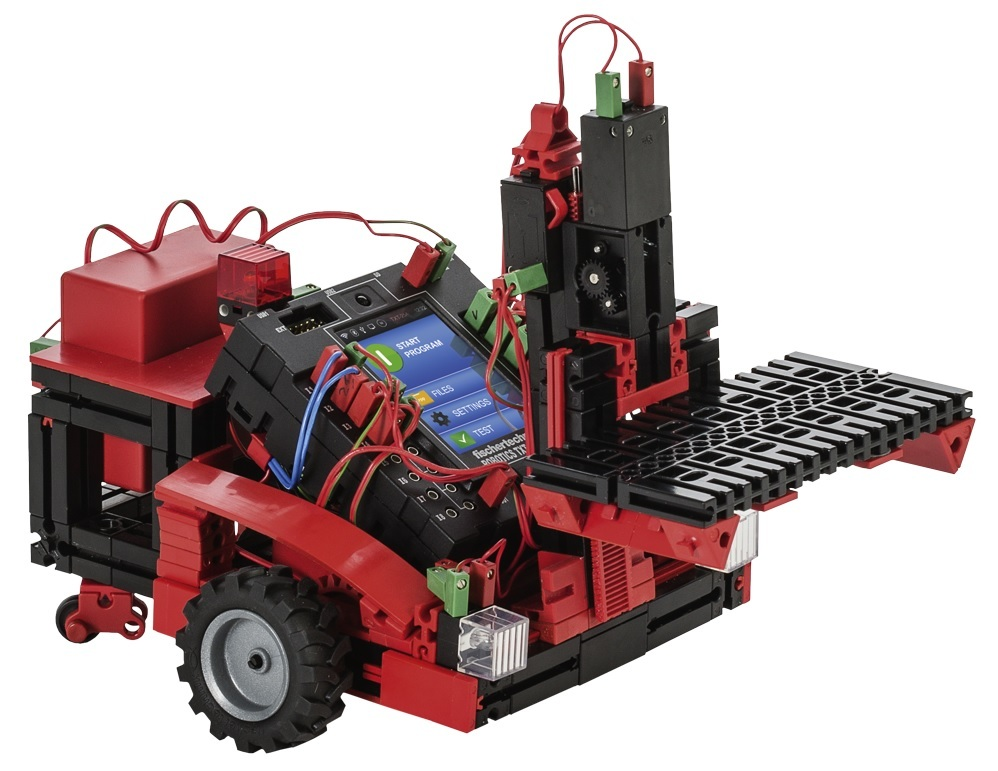
\includegraphics[width=300px]{images/fischertechnik_ROBO-TX-Explorer_02.jpg}
% 	\caption[Fischertechnik - ROBO TX Explorer]{Fischertechnik - ROBO TX Explorer \footnote{Zdroj: \url{http://www.helago-cz.cz/eshop-519143-workstation-robo-tx-training-lab-tx-explorer-146560.html}}
% \end{minipage}
% \end{figure}

% figure + footnote -> afterpage
% src: http://tex.stackexchange.com/questions/10181/using-footnote-in-a-figures-caption
%\afterpage{
%	\begin{figure}[h]
%	 	\centering
%		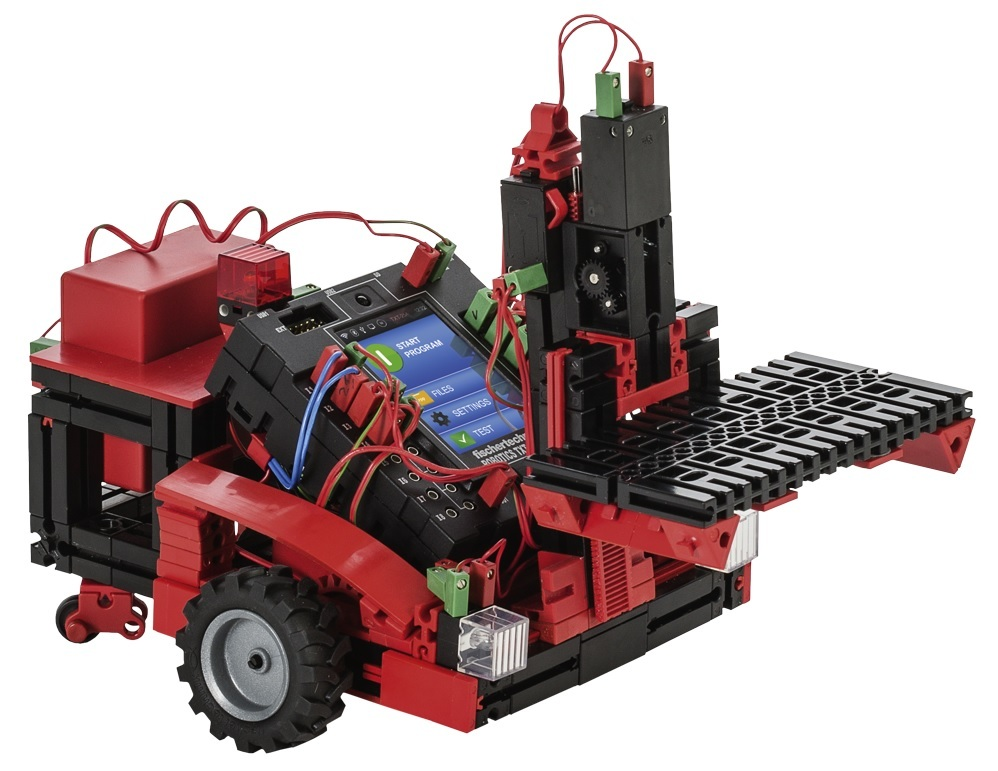
\includegraphics[width=300px]{images/fischertechnik_ROBO-TX-Explorer_02.jpg}
%			\caption[Fischertechnik - ROBO TX Explorer]{Fischertechnik - ROBO TX Explorer \footnotemark}
%		\label{fig:fischertechnik_ROBO-TX-Explorer}
%	\end{figure}
%	\footnotetext{Zdroj: \url{http://www.helago-cz.cz/eshop-519143-workstation-robo-tx-training-lab-tx-explorer-146560.html}}
%}

\begin{figure}[h]
	\centering
	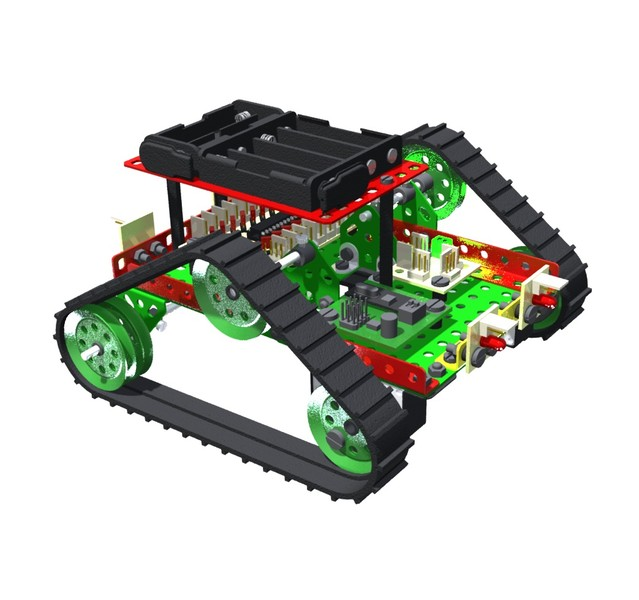
\includegraphics[width=235px]{images/MERKUR_Pasovy-podvozek-01_ATMEL+RC.jpg}
	\caption[MERKUR -- Pásový podvozek 01 -- ATMEL + RC]{MERKUR -- Pásový podvozek 01 -- ATMEL + RC\protect\footnotemark}
	\label{fig:MERKUR_Pasovy-podvozek-01_ATMEL+RC}
\end{figure}

\footnotetext{Zdroj: \url{http://www.merkurtoys.cz/vyrobky/pasovy-podvozek-merkur-s-elektronikou-rc}} 

Další zajímavou stavebnicí jsou Robotické sety od \merkur{u}~\cite{merkur_roboticsSetsEshop}. 
Nabídka jednotlivých setů je relativně široká a v porovnání s \legoM{ }nebo \fischerT{ }nabízí ještě bližší kontakt s elektronikou a samotným hardwarem. 
Jako řídicí mikrokontroléry můžete využít PIC nebo megaAVR od firmy Microchip. 
% * <lucie.karmova@jcmm.cz> 2017-04-27T13:11:10.851Z:
% 
% > řídící
% Správně řídicí, viz http://prirucka.ujc.cas.cz/?id=750
% 
% ^ <paral.jarek@gmail.com> 2017-04-27T13:26:35.414Z:
%
% Opraveno.
%
% ^ <paral.jarek@gmail.com> 2017-04-27T14:00:35.020Z.
Vzhledem k použitým procesorům je možné tyto stroje programovat v C/C++, PICAXE BASIC nebo i v grafickém prostředí~\cite{picaxeCz_BlocklyForPICAXE}. 
Robotické stavebnice od Merkuru mají podobné \uv{problémy} jako \fischerT. 
Kladou na uživatele větší nároky, nemají tak zvučnou značku, mají omezenější základní sadu senzorů a neumožňují tak rychlou stavbu fungujícího robota.

Na závěr lze zmínit výukové roboty, kteří jsou primárně, na rozdíl od robotických stavebnic, zaměřeny na velmi úzkou oblast činností (jízda po čáře, plnění jednoduchých sekvenčních úkolů, \dots). 
Tyto roboty jsou zajímavé z pohledu ceny, ale i jednoduššího využití ve výuce (žáci nemusí sestavovat konstrukci a hardware je plně připraven k používání). 
% * <lucie.karmova@jcmm.cz> 2017-04-27T13:16:27.168Z:
% 
% > Tito roboti
% Jednak tu nesedí podmět a přísudek (roboti jsou zajímavé), jednak v předchozím odstavci používáš neživotný tvar (roboty jsou zaměřeny).  Správně je obojí, ale měl by ses rozhodnout pro jeden tvar a ten pak v celém textu doržovat.
% 
% Viz http://vtm.e15.cz/aktuality/roboti-nebo-roboty-jazykova-anketa
% 
% ^ <paral.jarek@gmail.com> 2017-04-27T13:28:29.812Z:
%
% Pokus o opravu. Je to takhle dobře? :-|
%
% ^.
Naopak již neumožňují rozvoj kreativity studentů při stavbě a přizpůsobení robota pro různé soutěže (většinou je lze využívat jen v jedné soutěžní kategorii).  
Mezi takovéto roboty patří například Pololu 3pi~\cite{robotPololu3pi} (primárně určen pro jízdu po čáře -- zvládá jezdit až 1 m/s) nebo Edison~\cite{robotEdison} (umí sledovat čáru, lze jej programovat graficky i v Pythonu, má různé senzory, je možné jej kombinovat s \lego{ }kostkami). 
% * <lucie.karmova@jcmm.cz> 2017-04-27T13:18:50.401Z:
% 
% > patři 
% patří
% 
% ^ <paral.jarek@gmail.com> 2017-04-27T13:31:08.203Z:
%
% Opraveno.
%
% ^ <paral.jarek@gmail.com> 2017-04-27T14:01:09.210Z.
Tito roboti ovšem neumožňují takový rozsah činností jako \legoM.

\begin{figure}[h]
	\begin{minipage}[b]{.5\textwidth}
		\centering
		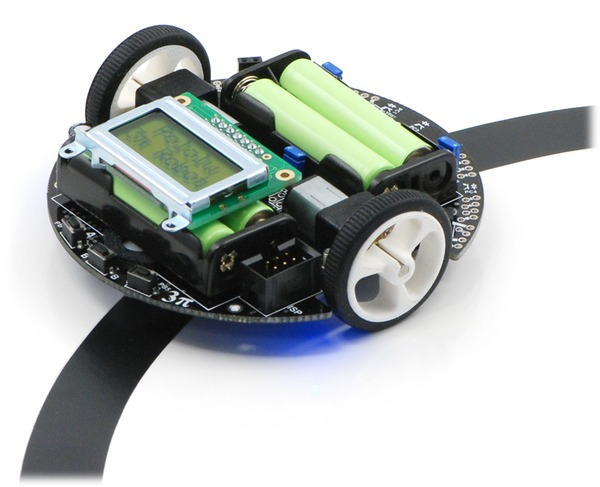
\includegraphics[width=\textwidth]{images/pololu-3pi-robot-8-on-line.jpg}
		\caption[Robot Pololu 3pi]{Robot Pololu 3pi\protect\footnotemark}
		\label{fig:pololu-3pi-robot-8-on-line}
	\end{minipage}
	\hfill
	\begin{minipage}[b]{.5\textwidth}
		\centering
		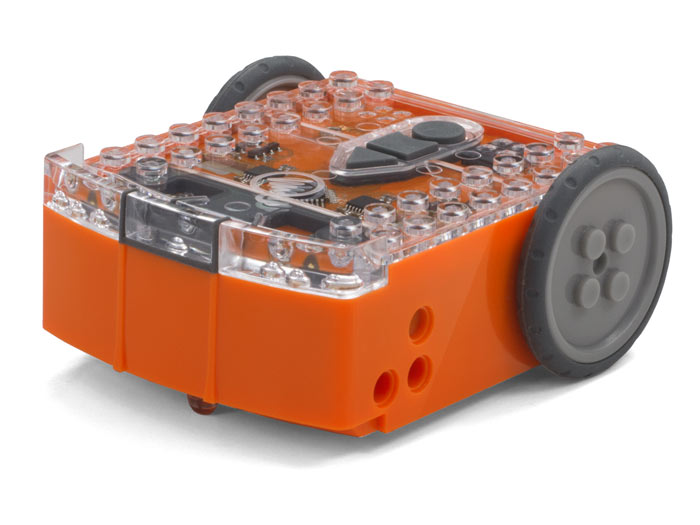
\includegraphics[width=\textwidth]{images/Edison-Educational-robot.jpg}
		\caption[Robot Edison]{Robot Edison\protect\footnotemark}
		\label{fig:Edison-Educational-robot}
	\end{minipage}
\end{figure}

% two footnote/footnotemark in minipage - problem with index
% solution: http://tex.stackexchange.com/a/43694

\addtocounter{footnote}{-1} % footnote_cnt -= 1
\footnotetext{Zdroj: \url{https://www.pololu.com/product/975}}
\stepcounter{footnote}
\footnotetext{Zdroj: \url{https://meetedison.com/meet-edison-v2-0/}}


% putting two images beside each other
% source: http://tex.stackexchange.com/a/148445

%\begin{figure}[!tbp]
%	\begin{subfigure}[b]{.5\textwidth}
%		\centering
%		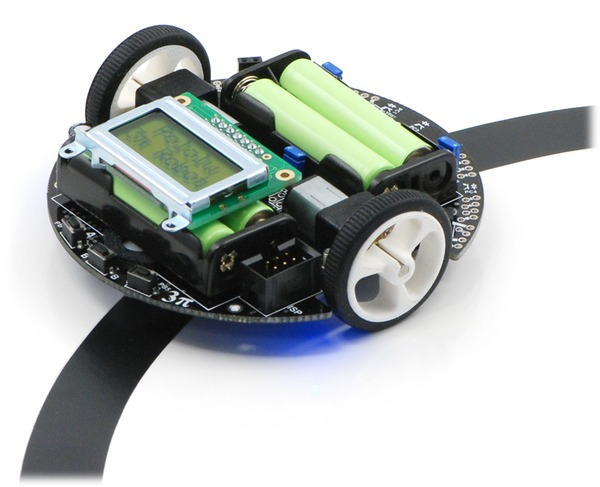
\includegraphics[width=\textwidth]{images/pololu-3pi-robot-8-on-line.jpg}
%		\caption[Robot Pololu 3pi]{Robot Pololu 3pi\protect\footnotemark}
%		\label{fig:pololu-3pi-robot-8-on-line}
%	\end{subfigure}
%	\hfill
%	\begin{subfigure}[b]{.5\textwidth}
%		\centering
%		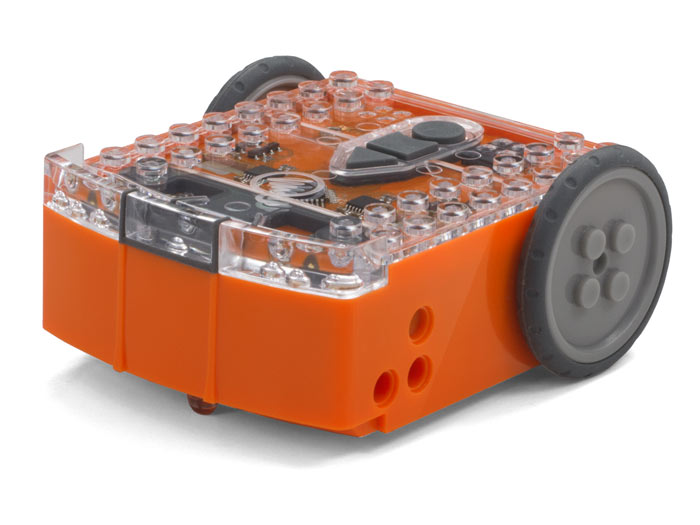
\includegraphics[width=\textwidth]{images/Edison-Educational-robot.jpg}
%		\caption[Robot Edison]{Robot Edison\protect\footnotemark}
%		\label{fig:Edison-Educational-robot}
%	\end{subfigure}
%	\caption{Roboti se zaměřením na velmi úzkou oblast činnost}
%\end{figure}
%
%\footnotetext{Zdroj: \url{https://www.pololu.com/product/975}} 
%\footnotetext{Zdroj: \url{https://meetedison.com/meet-edison-v2-0/}} 

\section{Motivace autora}

Již čtvrtým rokem vedu robotický kroužek na své bývalé střední škole SPŠ a VOŠ Brno, Sokolská a zároveň organizuji tábory a další vzdělávací akce v oblasti techniky a robotiky na pobočce Robotárna, Dům děti a mládeže Brno, Helceletova.
Už na střední škole jsem se v rámci těchto dvou organizací účastnil různých soutěží, jako například Robotický den v Praze, Mikrokontroléry letí na FEKT VUT Brno nebo Středoškolská odborná činnost (obory strojírenství a elektrotechnika). 
Z některých soutěží jsem si dovezl cenná umístění, ale i mnoho zkušeností, inspirace a podnětů na přemýšlení.
% * <lucie.karmova@jcmm.cz> 2017-04-27T13:22:45.206Z:
% 
% > podmětů
% Správně podnět. Podmět je ve větě s přísudkem :-)
% 
% ^ <paral.jarek@gmail.com> 2017-04-27T13:32:15.551Z:
%
% Opraveno.
%
% ^ <paral.jarek@gmail.com> 2017-04-27T14:00:29.943Z.

Za dobu, kterou se věnuji programování mikrokontrolérů a robotice, jsem již narazil na mnoho překážek a problémů, které bylo třeba překonat. 
%si už mnohokrát prošel trnitou cestou 
Tyto překážky jsou ovšem výrazně náročnější pro studenty, kteří v těchto oblastech teprve začínají a seznamují se s~nimi. 
% * <lucie.karmova@jcmm.cz> 2017-04-27T13:24:35.790Z:
% 
% > ní
% S oblastmi, s nimi.
% 
% ^ <lucie.karmova@jcmm.cz> 2017-04-27T13:25:09.916Z:
%
% Nebo v této oblasti, s ní
%
% ^ <paral.jarek@gmail.com> 2017-04-27T13:33:55.244Z:
%
% Snad opraveno :-).
%
% ^ <paral.jarek@gmail.com> 2017-04-27T20:37:01.761Z.
Často může nastat i situace, kdy je student se zájmem o robotiku odrazen její počáteční složitostí.
% * <lucie.karmova@jcmm.cz> 2017-04-27T13:25:27.379Z:
% 
% > , je odrazen
% ... kdy je student se zájmem o robotiku odrazen její počáteční složitostí
% 
% ^ <paral.jarek@gmail.com> 2017-04-27T13:35:21.864Z:
%
% Použito.
%
% ^ <paral.jarek@gmail.com> 2017-04-27T14:00:25.810Z.
Přitom by z něj mohl být v budoucnu perfektní programátor. 
Jen mu zrovna tenhle mikrokontrolér nejde naprogramovat nebo mu koupený H-můstek nechce roztočit motor.

Proto se svým studentům vždy snažím nachystat co nejlepší prostředí pro začátky s~robotikou. 
% * <lucie.karmova@jcmm.cz> 2017-04-27T13:26:48.603Z:
% 
% > s
% Jejky, na konci řádku! A o tři řádky níž zase.
% 
% ^ <paral.jarek@gmail.com> 2017-04-27T13:38:39.873Z:
%
% Na tohle se zatím nedívej, to vyřeší další nástroj pro LaTeX, který se jmenuje vlna (přidává do zdrojáku automaticky vlnky => ~ = nedělitelné mezery :-) ).
%
% ^.
Již jsem zkoušel různé platformy (například využít k výuce robota Pololu~3pi) i~způsoby výuky (kombinace elektroniky, programování na PC a~programování mikrokontrolérů), ale~bohužel vždy jsem se dostal do stejné situace. 
% * <lucie.karmova@jcmm.cz> 2017-04-27T13:27:19.963Z:
% 
% > elektroniku
% elektroniky?
% 
% ^ <paral.jarek@gmail.com> 2017-04-27T13:40:39.257Z:
%
% Opraveno.
%
% ^ <paral.jarek@gmail.com> 2017-04-27T13:54:55.518Z.
Ačkoliv mi studenti chodili již rok do robotického kroužku, pořád je dělily minimálně dva roky od schopnosti postavit a~naprogramovat složitějšího robota (s tím, že by použili předpřipravenou elektroniku, ale rozuměli tomu, co je jak zapojeno + uměli použít dostupné knihovny a naprogramovat si chování svého robota).
% * <lucie.karmova@jcmm.cz> 2017-04-27T13:27:48.255Z:
% 
% > dělili 
% Roky dělilY
% 
% ^ <paral.jarek@gmail.com> 2017-04-27T13:42:03.647Z:
%
% Opraveno.
%
% ^ <paral.jarek@gmail.com> 2017-04-27T13:47:29.691Z.

Nedávno jsme ale do kroužku zakoupili \legoEV{}. 
Stavebnici, která mi měla umožnit postavit robota za den. 
Prakticky stavebnice snů. No není to nádherná představa?
A~opravdu tomu tak bylo. Robota jezdícího po čáře jsme s manuálem zvládli poskládat a~zprovoznit za den. 
Studenti nemuseli studovat a řešit zapojení jednotlivých komponentů do řídicí elektroniky. 
% * <lucie.karmova@jcmm.cz> 2017-04-27T13:28:41.275Z:
% 
% > řídící 
% řídicí, důvod viz výše
% 
% ^ <paral.jarek@gmail.com> 2017-04-27T13:47:20.211Z:
%
% Opraveno.
%
% ^ <paral.jarek@gmail.com> 2017-04-27T13:47:31.076Z.
Nebylo třeba trávit mnoho času vysvětlováním způsobu programování 8bitových mikrokontrolérů (omezení paměti a výkonu, menší datové typy -- \verb|uint_8t|, komunikace po sériové lince, \dots).
% * <lucie.karmova@jcmm.cz> 2017-04-27T13:30:19.125Z:
% 
% > \dots
% Vypadá to jako tři tečky, určitě je to trojtečka?
% 
% ^ <paral.jarek@gmail.com> 2017-04-27T13:54:49.335Z:
%
% Už jsem to i před tím hledal a asi je tohle ta správná trojtečka. Zkusím to ještě probrat s kluky.
%
% ^ <paral.jarek@gmail.com> 2017-04-27T20:33:16.117Z:
%
% Je to takhle správně. Ještě lze použít \ldots, ale v textu by to mělo fungovat prakticky stejně.
%
% ^ <paral.jarek@gmail.com> 2017-04-27T20:33:17.632Z.
% * <lucie.karmova@jcmm.cz> 2017-04-27T13:29:27.176Z:
% 
% > 8bitových
% Jestli to není terminus technikus, určo se má psát 8bitových
% 
% ^ <paral.jarek@gmail.com> 2017-04-27T13:58:46.495Z:
%
% No nevím co to je nebo není, ale dost často se ta na českých webech píše s pomlčkou:
% http://www.fi.muni.cz/usr/jkucera/pv109/2000/vitek_atari.htmlhttp://www.sallyx.org/sally/zajem/intel.php
% http://www.8bity.cz/
% Ale na Wikipedii je 8bitový počítač: https://cs.wikipedia.org/wiki/8bitov%C3%BD
% Tak nevím :-|
%
% ^ <paral.jarek@gmail.com> 2017-04-27T15:23:57.837Z:
% 
% Nevíš, jestli je nějaká stránka, která mi řekne četnost daného slova v textech? Nemůžu nic najít, ale měl jsem za to, že něco takového existuje.
% 
% ^ <paral.jarek@gmail.com> 2017-04-27T20:33:32.513Z:
%
% Upraveno.
%
% ^ <paral.jarek@gmail.com> 2017-04-27T20:33:59.439Z.
Jen si poskládali z \lega{ }hardware, pomocí kabelů (které nelze otočit ani zapojit špatně a tím něco zničit) spojili jednotlivé moduly. 
% * <lucie.karmova@jcmm.cz> 2017-04-27T13:31:14.671Z:
% 
% > \lega{ }
% Ponechej všude LEGO a neskloňuj. Ono se to dobře vyslovuje, ale je to podobně špatně jako jet do IKEI (správně IKEA).
% 
% ^ <lucie.karmova@jcmm.cz> 2017-04-27T13:32:25.089Z:
%
% Viz http://prirucka.ujc.cas.cz/?id=398
%
% ^ <paral.jarek@gmail.com> 2017-04-27T14:06:36.340Z:
%
% Dobře. Opraveno.
%
% ^ <paral.jarek@gmail.com> 2017-04-27T14:06:38.211Z.
A~v~grafickém prostředí si poskládali svůj program.

Pak jsme se ale začali soustředit na zlepšování softwaru i hardwaru tak, abychom využili stavebnici na 100~procent, a v ten moment jsme narazili.
% * <lucie.karmova@jcmm.cz> 2017-04-27T13:37:20.359Z:
% 
% > procent a v ten
% 
% Před "a v ten moment" patří čárka,  viz http://prirucka.ujc.cas.cz/?id=153
% 
% ^ <paral.jarek@gmail.com> 2017-04-27T14:08:50.447Z:
%
% Opraveno. Je tu kvůli tomu, že je to "Poměr stupňovací"?
%
% ^. 
% * <lucie.karmova@jcmm.cz> 2017-04-27T13:36:35.845Z:
% 
% > softwaru i hardwaru, tak abychom 
% 
% Správně: softwaru i hardwaru tak, aby
% 
% ^ <paral.jarek@gmail.com> 2017-04-27T14:10:41.332Z:
% 
% Je to teď ok? Může tam zůstat "tak, abychom"? 
% 
% ^ <paral.jarek@gmail.com> 2017-04-27T20:35:08.075Z.

Dokud jsme si s EV3 jen \uv{hráli} a nesoustředili se primárně na výkon a spolehlivost, bylo vše v pořádku. 
Jakmile jsme ale chtěli mít regulační smyčku PID~regulace pro robota na sledování černé čáry s periodou 10~ms, zjistili jsme, že to nejde (a to máme v EV3 \brick{\it u} 300~MHz~ARM). Přitom díky předešlým zkušenostem s 8bitovými mikrokontroléry Atmel~AVR jsme věděli, že by to neměl být problém.
% * <lucie.karmova@jcmm.cz> 2017-04-27T13:38:31.798Z:
% 
% > 8bitovými
% Viz výše
% 
% ^ <paral.jarek@gmail.com> 2017-04-27T14:11:38.625Z:
%
% Viz výše.
%
% ^ <paral.jarek@gmail.com> 2017-04-27T20:36:41.598Z.

To samé platí o grafickém vývojovém prostředí dodávaném s \EVthree. Dokud máte na obrazovce několik programových bloků, vše funguje bez problémů. 
Když se však program rozroste na několik obrazovek a samostatných modulů, velmi rychle ztrácíte přehlednost a efektivitu programování.
Zároveň vám již moc nepomohou ladicí nástroje, které jsou součástí prostředí, protože při jednoduchém programu je lze relativně dobře využít, ale při rozsáhlejších programech již nejsou k dispozici nebo je jejich použití velmi komplikované. 
% * <lucie.karmova@jcmm.cz> 2017-04-27T13:39:18.667Z:
% 
% >  ladící
% Ladicí, viz výše
% 
% ^ <paral.jarek@gmail.com> 2017-04-27T14:11:59.053Z:
%
% Opraveno.
%
% ^ <paral.jarek@gmail.com> 2017-04-27T14:12:26.457Z.

Proto jsme začali hledat alternativní platformy, které by odstraňovaly zmíněné problémy, což vyústilo v tuto práci.   
% * <lucie.karmova@jcmm.cz> 2017-04-27T13:40:18.126Z:
% 
% > platformy, které by odstraňovali
% 
% Správně: Platformy by odstraňovalY
% 
% ^ <paral.jarek@gmail.com> 2017-04-27T14:12:25.098Z:
%
% Opraveno.
%
% ^ <paral.jarek@gmail.com> 2017-04-27T14:14:24.062Z.
